\documentclass[12pt]{report}
\usepackage{blindtext}
\usepackage{hyperref}
\usepackage{tocloft}
\usepackage{natbib}
\usepackage{graphicx}
\usepackage[newfloat]{minted}
\usepackage{caption}
\newenvironment{longlisting}{\captionsetup{type=listing}}{}
\title{%
  Neural Network, Genetic Algorithm,\\
  Robot Algorithm Creation Report\\
  \large IMAT2801 CI and Control Systems \\
    De Montfort University}
\author{Artem Bobrov (P2547788)}
\date{May 15 2021}
\setlength{\parindent}{1em}
\begin{document}
\maketitle
\thispagestyle{empty}
\clearpage
\tableofcontents
\setcounter{tocdepth}{1}
\thispagestyle{empty}
\clearpage
\section*{Introduction}
\addcontentsline{toc}{section}{Introduction}

\paragraph{}
% Introduction text

\textbf{Computational Intelligence} and \textbf{Control Systems} began to gain popularity with unbelievable rates. Having said that both of them are intended for problem solving yet they are quite different. 

\textbf{Computational Intelligence} introduced the ability of computers to "learn" and use given information (datasets) to solve specific problems. It can be used to fulfil simple tasks such as training it on a small datasets
(this was accomplished within this project), as well as more complicated problems like monitoring the haloketones presence in drinking water. It is believed that linear/log regressions models cannot well predict haloketone levels
but backpropagation algorithm is good to predict haloketone levels in internal validation \citep{BPArticle1}. %(Y. Deng et al. 2021).

\textbf{Control Systems} on the other hand are mostly used to regulate problems on a physical layer. For example a control system can affect the behaviour of another device based on the gathered information.
A simple example is a thermostat controlling a boiler. A maze-solving algorithm is a part of control systems. It is believed that needs in a control system that can control a robot in an efficient way are growing \citep{RobotArticle1}. %(H. Dang et al. 2010)
\\

This report provides information and description of the working process carried out in order to complete the coursework for \textbf{IMAT2801 CI and Control Systems}. Three tasks that were to be undertaken are:
\begin{itemize}
  \item Neural Network with backpropagation mechanism 
  \item Genetic Algorithm
  \item Maze-solving robot in CoppeliaSim
\end{itemize}

All three tasks required not only good knowledge of programming languages such as \textbf{Python} and \textbf{Lua} but also a well thought out design of those complex programs.


\clearpage

\section*{Neural Network solution (written in Python)}
\addcontentsline{toc}{section}{Neural Network solution (written in Python)}

\subsection*{Overview}
\addcontentsline{toc}{subsection}{Overview}
\paragraph{}

The neural network created for this assignment features a backpropagation mechanism and is a feedforward type of a network. Backpropagation is a basic tool for pattern classification application of Artifical
Neural Networks medical diagnosis and remote sensing \citep{NNArticle1}. In spite of the fact that this neural network is not used for medical researches, backpropagation plays a big role in all-purpose ANNs.
In simpler terms backpropagation refers only to the algorithm for computing the gradient \citep{wiki:Backpropagation}. Neural networks mimic the human brains and neuron connections specifically. Human learning
reflects on the connections between neurons and changes the strength of the bonds between them. Neural networks use term "weights" to describe the strength of these bonds \citep{NNArticle1}.


\subsection*{Coding}
\addcontentsline{toc}{subsection}{Coding}
\paragraph{}

% Coding explanation

%\clearpage

\subsection*{Results}
\addcontentsline{toc}{subsection}{Results}
\paragraph{}

% Results info (GIFs, pictures, outcomes, screenshots)

\clearpage

\section*{Genetic Algorithm (written in Python)}
\addcontentsline{toc}{section}{Genetic Algorithm (written in Python)}

\subsection*{Overview}
\addcontentsline{toc}{subsection}{Overview}
\paragraph{}

\textbf{Genetic Algorithms} are a part of evolutionary computing and biological theory is used as a base in their design. They are used to solve different optimisation problems as well as search problems.
Those algorithms mimic the principles of nature. Survival of the fittest is the main goal of genetic algorithms. Yet not all of them stick to the same rule. There are some other genetic algorithms called nomadic
which do not discard the weakest species \citep{GeneticAlgorithmArticle1}.

The assigned task was to design a genetic algorithm for \textbf{Ackley Function} optimisation. The algorithm in the appendix 2 introduces a mutation function
in order to maintain genetic diversity between the generations. Respectively, it follows the principles of the biological mutation.

\subsection*{Coding}
\addcontentsline{toc}{subsection}{Coding}
\paragraph{}

The genetic algorithm solution is written in \textbf{Python} and PyCharm IDE by JetBrains was used in order to complete the task.
The whole project was split in separate classes (and different files) to maintain code readability and maintainability.
Random and Math libraries were used during creation of this project. The genetic algorithm is made universal and can work with
every given function. Passed a number of tests for a sphere function and Ackley Function. Planned tests include: Rastrigin function, 
Rosenbrock function.

Difficulties: Mutation function was quite complex to implement and designing the offset change in particular.
The main complexity in writing the code was to translate every rule and thought into code.


\subsection*{Results}
\addcontentsline{toc}{subsection}{Results}
\paragraph{}

Created genetic algorithm was tested optimising Ackley Function and it showed the following results: -0.06783551718545366 as for the X coordinate, -0.014311762013534637 as for the Y coordinate and 0.31929690272986244 as for the best score value with
parameters as follows: number of individuals = 500, crossover rate = 0.5, mutation steps = 15, chance of mutation = 0.4, number of epochs = 15, result limited between -5 and 5.
Those results can vary in different runs and iterations therefore allow some difference.

\clearpage

\section*{Maze-solving Algorithm (written in Lua)} % Lighting, Physical Sky
\addcontentsline{toc}{section}{Maze-solving Algorithm (written in Lua)}

\subsection*{Overview}
\addcontentsline{toc}{subsection}{Overview}
\paragraph{}

Robots are essential in science and especially in undertaking tasks that are impossible to be accomplished by a human being. The task set by the assignment was related to designing
the behaviour of the pioneer robot which can be used to explore, document, transport, research and many other things. In order the robot to work properly it has to be programmed for
a specific task. 

The main algorithm of the robot presented in this report was to solve a given maze. In the presented code it runs a modified Breitenberg algorithm that uses multipliers to control
velocity of the wheels and an additional variable used to detect a wall in front of it.

\subsection*{Coding}
\addcontentsline{toc}{subsection}{Coding}
\paragraph{}

The code features a state machine using an improvisation in order to mimic a switch statement present in other programming languages (e.g. C++, Java, PHP). We have a set of states which correspond to
the robot's current action. Multipliers are used to control the velcity of the motors so the turns can be manipulated precisely. In the initialisation function the lab "skeleton" was used to 
facilitate the coding.

Difficulties: Many maze-solving algorithm were applied but not implemented correctly in Lua. Wall-following Algorithm, Left-hand Algorithm, standard Breitenberg Algorithm among
others were applied with no success.

\clearpage

\subsection*{Results}
\addcontentsline{toc}{subsection}{Results}
\paragraph{}

The robot (P3DX model) had a task to complete the maze without being hard-coded to do so. The time is not recorded with a command but is displayed with a built-in graph object in CoppeliaSim "attached" to the robot.
The graph below shows the time taken by the robot to complete the maze. As it can be seen, the time taken is approximately 80 seconds.
The pioneer follows a "right-hand" algorithm as if there's space it turns right. If not right, then left. The robot doesn't store any information about visited tiles and follows a simpler set of instructions.

\begin{figure} [!h]
  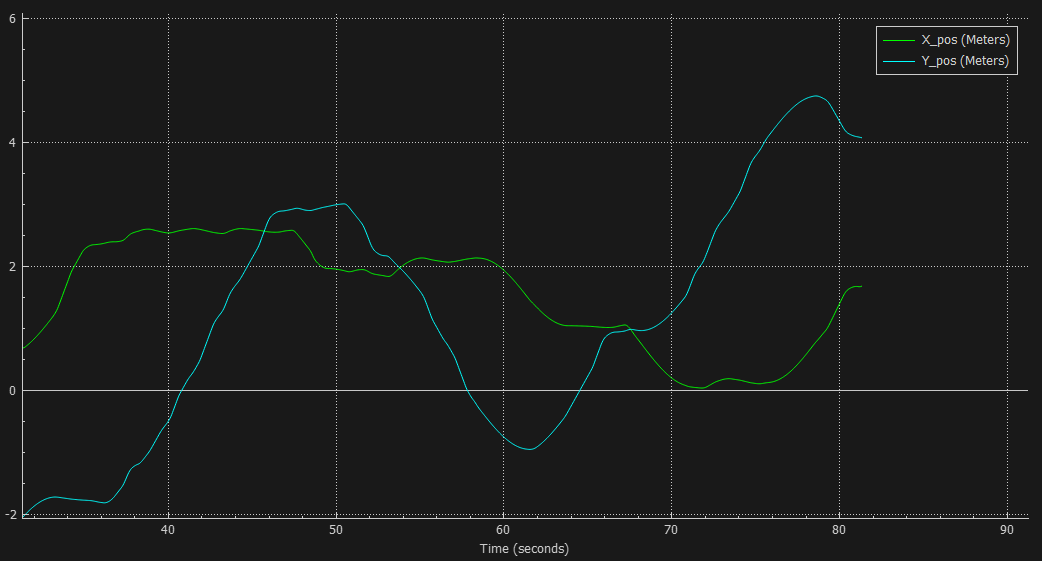
\includegraphics[width=\linewidth]{graph.png}
  \caption{A graph showing the absolute position relation to time.}
  \label{fig:boat1}
\end{figure}

The robot has been tested multiple amount of time in the given maze only and it's not certain that it will be able to solve other more complex mazes but it's believed that the algorithm is modifiable and can be used as a base in creating more
complicated systems to solve more complicated problems (mazes). An attempt was made to use a "left-hand" algorithm to solve the given maze but the peciluliar properties of this maze didn't allow the "left-hand" algorithm. The first turn in the maze
has a catch and is very hard to solve by a robot using only its supersonic sensors to scan the environment.
\clearpage

\section*{Conclusion}
\addcontentsline{toc}{section}{Conclusion}

% Conclusion text

\clearpage


\section*{Appendix 1 - NN Code}
\addcontentsline{toc}{section}{Appendix 1 - NN Code}
\paragraph{}

% NN Code

\clearpage

\section*{Appendix 2 - GA Code}
\addcontentsline{toc}{section}{Appendix 2 - GA Code}
\paragraph{}

% GA Code

\clearpage

\section*{Appendix 3 - Robot Code}
\addcontentsline{toc}{section}{Appendix 3 - Robot Code}
\paragraph{}

% Robot Code
\begin{longlisting}
\inputminted[linenos,breaklines]{lua}{code/leftHand.lua}
\end{longlisting}

\clearpage

\addcontentsline{toc}{section}{Bibliography}
\bibliography{reference}{}
\bibliographystyle{agsm}
\end{document}